\label{section:1d_hillslope_example}
The examples \texttt{3\_0\_SWF\_CHD}, \texttt{3\_1\_CLN\_for\_SWF} and \texttt{3\_SWF} simulate 1D surface flow on a 100 m long, 1 m wide sloping surface.  Analytical and
numerical solutions of the diffusive wave and dynamic wave equations for this problem were presented by Govindaraju
et al. (1988a,b).

The first two examples compare surface flow in a \swf\ domain (\texttt{3\_0\_SWF\_CHD}) versus an equivalent \cln\ domain (\texttt{3\_1\_CLN\_for\_SWF}). For the \swf\ domain, the following parameter values were used:

\begin{center}
    \begin{tabular}{lll}  \hline
        Parameter                           & Value                     &   Unit            \\ \hline
        Manning's coefficient               &  $5.48 \times 10^{-2}$    &   s m$^{-1/3}$   \\
        Depression storage height           &  0.1                      &   m               \\
        Obstruction storage height          &  0.0                      &   m               \\
        Depth for smoothing height 1        &  $1 \times 10^{-6}$       &   m               \\
        Depth for smoothing height 2        &  $1 \times 10^{-6}$       &   m               \\
    \hline
    \end{tabular}
\end{center}


For the equivalent \cln\ domain, the following parameter values were used:

\begin{center}
    \begin{tabular}{lll}  \hline
        Parameter                               & Value                     &   Unit            \\ \hline
        Longitudinal hydraulic conductivity     &  $5.48 \times 10^{-2}$    &   m s$^{-1}$      \\
        Rectangular Width                       &  1.0                      &   m               \\
        Rectangular Height                      &  1.0                      &   m               \\
    \hline
    \end{tabular}
\end{center}

The \cln\ channel was assigned a rectangular geometry, a horizontal direction and assumed an unconfined/Mannings flow treatment.

The following parameter values were used for the \gwf\ domain in both cases, although interaction between the surface flow and \gwf\ domains was negligible due to the short simulation time of 242 seconds:

\begin{center}
    \begin{tabular}{lll}  \hline
        Parameter                     & Value & Unit                                \\ \hline
        Specific yield (porosity)     &  0.3                        &               \\
        Hydraulic conductivity        &  $ 1.474 \times 10^{-4}$    &   m s$^{-1}$  \\
        Specific storage coefficient  &  $ 1 \times 10^{-4}$        &   m$^{-1}$    \\
        Van Genuchten Alpha           &  1.0                        &   m$^{-1}$    \\
        Van Genuchten Beta            &  5                          &               \\
        Residual saturation           &  0.3                        &               \\
        Initial surface water depth   &  $1 \times 10^{-5}$         &   m           \\
    \hline
    \end{tabular}
\end{center}

The Van Genuchten unsaturated function type was used.

An initial surface water depth of $1 \times 10^{-6}$ m was assigned to the \swf\ and \cln\ surface flow domains.

Boundary conditions for the \swf\ and \cln\ surface flow domains consist of a flux of $4 \times 10^{-3}$ m/s applied to the entire domain and a specified head slightly above ground surface applied to the cell located at the downstream outflow boundary.

\pagebreak
Here is a comparison of outflow versus time (upper plot)  and surface water depth versus distance along the slope (lower plot) at the constant head cells for the \swf\ and \cln\ domains at the end of the simulation:

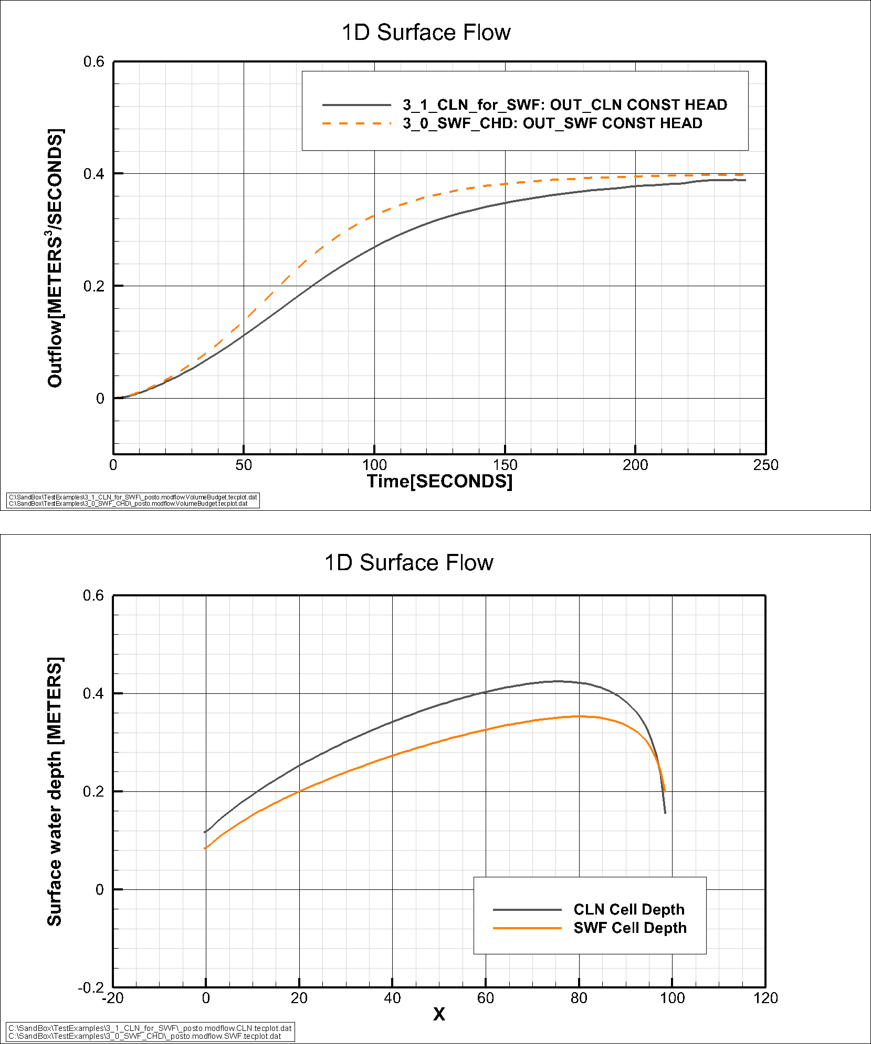
\includegraphics[width=0.87\textwidth]{5_3_OutflowDepthComparison}

Outflow builds up during the simulation and levels off at a value of 0.4 m$^{3}$/s (i.e. recharge rate times slope length).   Depths increase downstream then drop sharply approaching the constant head outlet cell.

\pagebreak
The third example (\texttt{3\_SWF}) is identical to the second example, except a critical depth boundary condition is applied to the \swf\ domain cell located at the downstream outflow boundary.

Here is a comparison of outflow versus time (upper plot) and surface water depth versus $x$ (i.e.\ distance along the slope) (lower plot) at the critical depth cells for the \mfus\ and \hgs\ models:

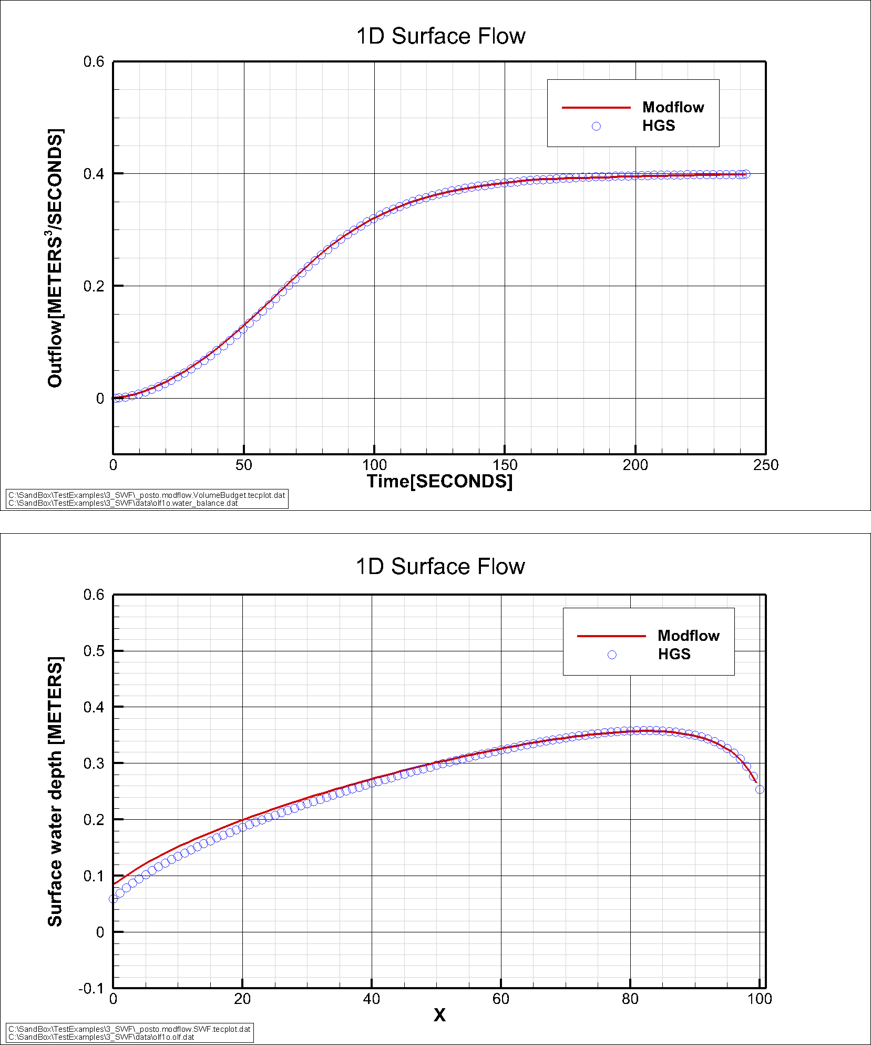
\includegraphics[width=0.87\textwidth]{5_4_OutflowDepthComparisonWithHGS.png}


